\documentclass[12pt, a4paper]{article}

% Codificacao e idioma
\usepackage[utf8]{inputenc}
\usepackage[T1]{fontenc}
\usepackage[brazil]{babel}

% Layout e margem ABNT
\usepackage[top=3cm, bottom=2cm, left=3cm, right=2cm]{geometry}

% Tipografia
\usepackage{times}
\usepackage{setspace}
\onehalfspacing

% Figuras e tabelas
\usepackage{graphicx}
\usepackage{float}
\usepackage{booktabs}
\usepackage{longtable}
\usepackage{array}

% Codigos
\usepackage{listings}
\usepackage{xcolor}

% Posicionamento absoluto (brasao da capa)
\usepackage{tikz}

% Links e referencias
\usepackage[hidelinks]{hyperref}
\usepackage[
  backend=biber,
  style=abnt,
  citestyle=abnt
]{biblatex}
\addbibresource{referencias.bib}

% Identacao do primeiro paragrafo
\usepackage{indentfirst}

% Titulos de secao
\setcounter{secnumdepth}{3}
\setcounter{tocdepth}{3}

% Configuracao de listings
\lstset{
  basicstyle=\ttfamily\small,
  breaklines=true,
  frame=single,
  backgroundcolor=\color{gray!10},
  captionpos=b
}

% -----------------------------------------------------------
\begin{document}

% -----------------------------------------------------------
% CAPA
% -----------------------------------------------------------
\begin{titlepage}
\newgeometry{top=2cm, bottom=2cm, left=2.5cm, right=2.5cm}

% Brasao em posicao absoluta (nao influencia o layout do texto)
\begin{tikzpicture}[remember picture, overlay]
  \node[anchor=north west, xshift=2.5cm, yshift=-2cm]
    at (current page.north west)
    {
\includegraphics[height=2.8cm]{figuras/brasao-unisantos.png}};
\end{tikzpicture}

\vspace*{1.2cm}

% Todas as 4 linhas centralizadas no mesmo eixo
\begin{center}
  {\large\bfseries UNIVERSIDADE CAT\'OLICA DE SANTOS}\\[0.3cm]
  {\large Ci\^encia da Computa\c{c}\~ao}
\end{center}

\vfill

\begin{center}
  {\fontsize{28}{34}\selectfont\bfseries Explora+}\\[0.8cm]
  {\large\bfseries Entrega de Prot\'otipo}
\end{center}

\vfill\vfill

% Autores alinhados a esquerda
\begin{flushleft}
{\large
  Felipe Barbosa dos Santos\\[0.3cm]
  Felipe de Lima Monteiro\\[0.3cm]
  Lucas Carmona Neto\\[0.3cm]
  Lucas Cerqueira Galv\~ao\\[0.3cm]
  Jo\~ao Gabriel Henriques Cardoso
}
\end{flushleft}

\vspace{1.8cm}

% Data centralizada no rodape
\begin{center}
  {\large Santos -- SP, junho de 2026}
\end{center}

\restoregeometry
\end{titlepage}

\thispagestyle{empty}
\tableofcontents
\newpage

% -----------------------------------------------------------
\section{Introdu\c{c}\~ao}
% -----------------------------------------------------------

O projeto Explora+ \'e uma iniciativa de extens\~ao desenvolvida por estudantes de Ci\^encia da Computa\c{c}\~ao da Universidade Cat\'olica de Santos com o objetivo de criar um aplicativo m\'ovel para promo\c{c}\~ao do turismo local.

\subsection{Problema}

Cidades de m\'edio porte como Santos -- SP possuem rico acervo tur\'istico e cultural, mas enfrentam baixa visibilidade de seus atrativos pela aus\^encia de ferramentas digitais acess\'iveis e integradas. Visitantes e moradores frequentemente desconhecem monumentos hist\'oricos, parques e pontos de interesse pr\'oximos, e n\~ao t\^em como planejar percursos tur\'isticos de forma autom\'atica.

\subsection{Solu\c{c}\~ao proposta}

O Explora+ oferece um planejador de rotas tur\'isticas que:

\begin{itemize}
  \item Calcula automaticamente um percurso pedestre entre dois pontos;
  \item Identifica pontos de interesse (POIs) pr\'oximos ao trajeto via dados abertos do OpenStreetMap;
  \item Enriquece os detalhes de cada POI com imagens e resumos buscados no Wikidata e Wikipedia;
  \item Permite ao usu\'ario marcar lugares como visitados, excluir paradas, manter uma biblioteca pessoal de lugares e configurar como a pr\'oxima busca de rota deve ser feita.
\end{itemize}

\subsection{Stakeholder externo}

O cliente externo do projeto \'e Felipe Pacheco Fernandes, ex-CRO do Grupo Costa Norte de Comunica\c{c}\~ao, sediado na Baixada Santista/SP. Ao longo do desenvolvimento, Felipe deixou o grupo em que estava inserido e passou a conduzir seu envolvimento com o projeto de forma independente, atuando como Product Owner externo \`a organiza\c{c}\~ao.

Essa mudan\c{c}a teve impacto direto na vis\~ao do produto: desvinculado de uma empresa com atuação regional específica, o PO ampliou o escopo conceitual do Explora+ de um app pensado para integrar parceiros comerciais da Baixada Santista para uma \textbf{plataforma de prop\'osito geral}, capaz de atender turistas de qualquer cidade com perfil tur\'istico semelhante ao de Santos. O produto passou a ser concebido como um aplicativo independente, com potencial de lan\c{c}amento e monetiza\c{c}\~ao aut\^onoma, sem depend\^encia de parcerias institucionais espec\'ificas para operar.

Esse reposicionamento est\'a alinhado com o car\'ater extensionista do projeto: a solu\c{c}\~ao desenvolvida aplica conhecimento acad\^emico para um problema real e transferível, com impacto potencial que ultrapassa o contexto local onde foi originada.

% -----------------------------------------------------------
\section{Desenvolvimento}
% -----------------------------------------------------------

\subsection{Metodologia e organiza\c{c}\~ao do time}

O time adotou metodologia \'agil com sprints semanais, organiza\c{c}\~ao de tarefas via Trello e reuni\~oes peri\'odicas com o Product Owner externo. O c\'odigo e a documenta\c{c}\~ao est\~ao p\'ublicos na organiza\c{c}\~ao GitHub \textbf{EXPLORA-PLUS} (\url{https://github.com/EXPLORA-PLUS}), estruturados em tr\^es reposit\'orios independentes:

\begin{itemize}
  \item \texttt{explora-plus-backend} -- API Django;
  \item \texttt{explora-plus-frontend} -- app Expo/React Native;
  \item \texttt{explora-plus-docs} -- documenta\c{c}\~ao, modelagem e paper.
\end{itemize}

\subsection{Proposta inicial de arquitetura}

No in\'icio do semestre, a arquitetura proposta previa integra\c{c}\~ao com APIs comerciais como Google Maps (geolocaliza\c{c}\~ao e roteamento), GeoAPIFy (backup de geocodifica\c{c}\~ao), Sympla e TicketMaster (eventos culturais), Uber e 99 (mobilidade urbana) e Quanto Tempo Falta (transporte p\'ublico). O modelo de dados inicial era centrado em uma entidade \texttt{Route} de destino \'unico (\emph{single-destination}). Essa proposta foi elaborada em um contexto em que o PO atuava dentro do Grupo Costa Norte, o que sugeria a viabilidade de parcerias com estabelecimentos comerciais e ag\^encias de turismo locais como suporte \`a distribui\c{c}\~ao do produto.

Com a mudan\c{c}a desse contexto -- e a consequente revis\~ao da vis\~ao do produto para uma plataforma independente -- a arquitetura foi revista para refletir uma abordagem mais aut\^onoma e escal\'avel, eliminando depend\^encias de APIs pagas e parceiros institucionais. As justificativas detalhadas est\~ao na Se\c{c}\~ao~\ref{sec:arch}.

\subsection{Arquitetura implementada}
\label{sec:arch}

\subsubsection{Stack tecnol\'ogico}

\begin{table}[H]
\centering
\caption{Stack tecnol\'ogico do Explora+}
\begin{tabular}{lll}
\toprule
\textbf{Camada} & \textbf{Tecnologia} & \textbf{Vers\~ao} \\
\midrule
Backend framework & Django + DRF & 5.1.4 / 3.15.2 \\
Autentica\c{c}\~ao & SimpleJWT & 5.3.1 \\
Banco de dados & PostgreSQL + PostGIS & 16 / 3.4 \\
Infraestrutura & Docker + Docker Compose & -- \\
Frontend framework & Expo + React Native & 52 / 0.76 \\
Linguagem frontend & TypeScript & -- \\
Mapa & Leaflet (via WebView/iframe) & -- \\
\bottomrule
\end{tabular}
\end{table}

\subsubsection{APIs externas utilizadas}

A decis\~ao de usar exclusivamente APIs gratuitas e abertas foi motivada por tr\^es fatores: (1) sustentabilidade do projeto sem custos de opera\c{c}\~ao; (2) disponibilidade imediata sem cadastro ou aprova\c{c}\~ao; (3) qualidade dos dados do OpenStreetMap para a regi\~ao de Santos.

\begin{table}[H]
\centering
\caption{APIs externas integradas}
\begin{tabular}{lll}
\toprule
\textbf{Servi\c{c}o} & \textbf{Papel} & \textbf{Substitui} \\
\midrule
Nominatim & Geocodifica\c{c}\~ao de endere\c{c}os & Google Maps / GeoAPIFy \\
OSRM & Roteamento pedestre & Google Maps Directions \\
Overpass API & Busca de POIs via OSM & Google Places \\
Wikidata API & Imagem principal do lugar (P18) & -- \\
Wikipedia REST API & Resumo descritivo e imagem fallback & -- \\
\bottomrule
\end{tabular}
\end{table}

O enriquecimento de detalhes de POI segue uma cadeia progressiva: Nominatim fornece endere\c{c}o e extratags OSM (que podem conter \texttt{wikidata} e \texttt{wikipedia}); Wikidata fornece imagem via propriedade P18; se n\~ao houver t\'itulo Wikipedia dispon\'ivel, o sistema pesquisa o Wikipedia por nome do lugar (primeiro em portugu\^es, depois em ingl\^es) como fallback \cite{nominatim2024, wikidata2024, wikipedia2024}.

\subsubsection{Diagrama de Componentes}

\begin{figure}[H]
  \centering
  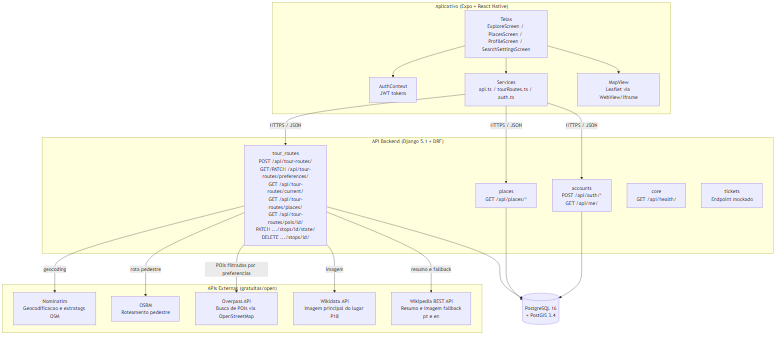
\includegraphics[width=0.95\textwidth]{figuras/componentes.png}
  \caption{Diagrama de componentes do Explora+}
\end{figure}

\subsubsection{Diagrama de Implanta\c{c}\~ao}

\begin{figure}[H]
  \centering
  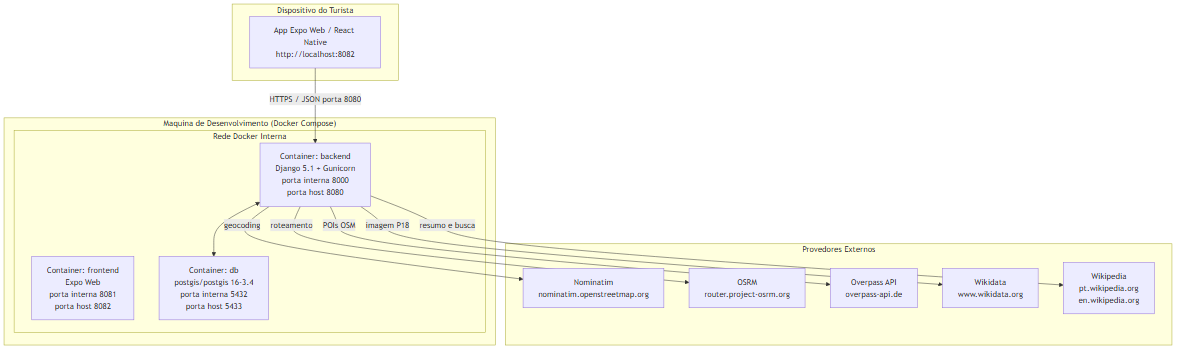
\includegraphics[width=0.85\textwidth]{figuras/implantacao.png}
  \caption{Diagrama de implanta\c{c}\~ao -- ambiente Docker de desenvolvimento}
\end{figure}

O ambiente de desenvolvimento usa Docker Compose com tr\^es containers: \texttt{backend} (Django + Gunicorn, porta 8080), \texttt{frontend} (Expo Web, porta 8082) e \texttt{db} (PostgreSQL + PostGIS, porta 5433) \cite{docker2024}.

\subsection{Modelagem de dados}

\subsubsection{Diagrama Entidade-Relacionamento}

\begin{figure}[H]
  \centering
  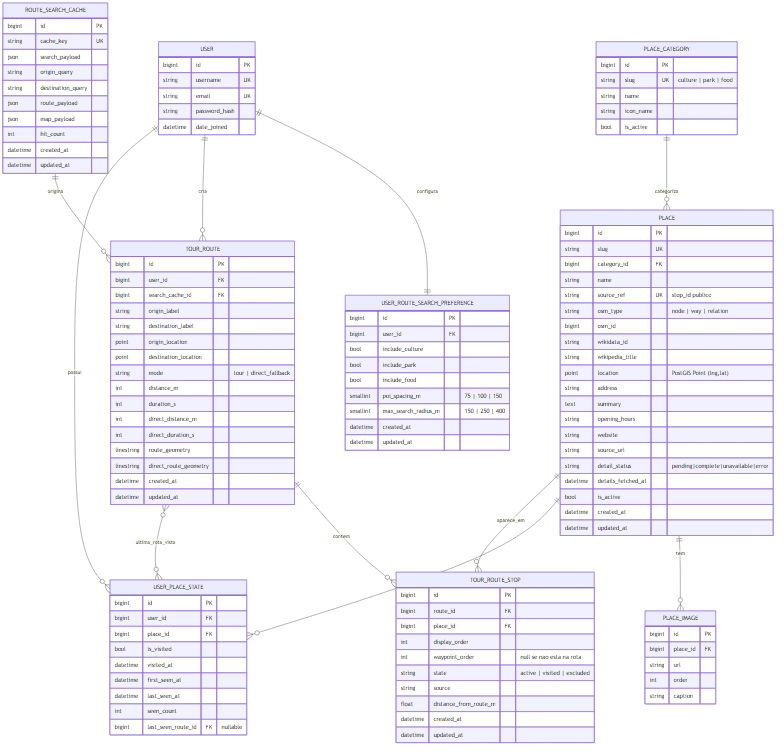
\includegraphics[width=0.95\textwidth]{figuras/er.png}
  \caption{Diagrama ER do Explora+ -- MVP entregue}
\end{figure}

O modelo de dados evoluiu significativamente em rela\c{c}\~ao \`a proposta inicial. A entidade \texttt{Route} de destino \'unico foi substitu\'ida por um conjunto de entidades que suportam rotas multi-POI e personaliza\c{c}\~ao por usu\'ario:

\begin{itemize}
  \item \textbf{UserRouteSearchPreference}: prefer\^encias persistidas do planner por usu\'ario autenticado. Controla categorias habilitadas, dist\^ancia alvo entre POIs e raio m\'aximo de elegibilidade.
  \item \textbf{Place}: fonte \'unica de verdade de um POI. Campo \texttt{source\_ref} \'e o identificador p\'ublico (\texttt{stop\_id} no contrato HTTP). Campo \texttt{detail\_status} controla o ciclo de enriquecimento progressivo.
  \item \textbf{UserPlaceState}: estado global do usu\'ario em rela\c{c}\~ao a um lugar (visitado, contagens, \'ultima rota em que apareceu).
  \item \textbf{RouteSearchCache}: cache de rota calculada por chave can\^onica (origem + destino + prefer\^encias efetivas). Evita recalcular via Nominatim/OSRM/Overpass a cada requisi\c{c}\~ao.
  \item \textbf{TourRoute}: snapshot relacional da rota personalizada do usu\'ario com geometria LineString PostGIS.
  \item \textbf{TourRouteStop}: cada POI na rota com estado \texttt{active / visited / excluded}.
\end{itemize}

\subsubsection{Diagrama de Classes}

\begin{figure}[H]
  \centering
  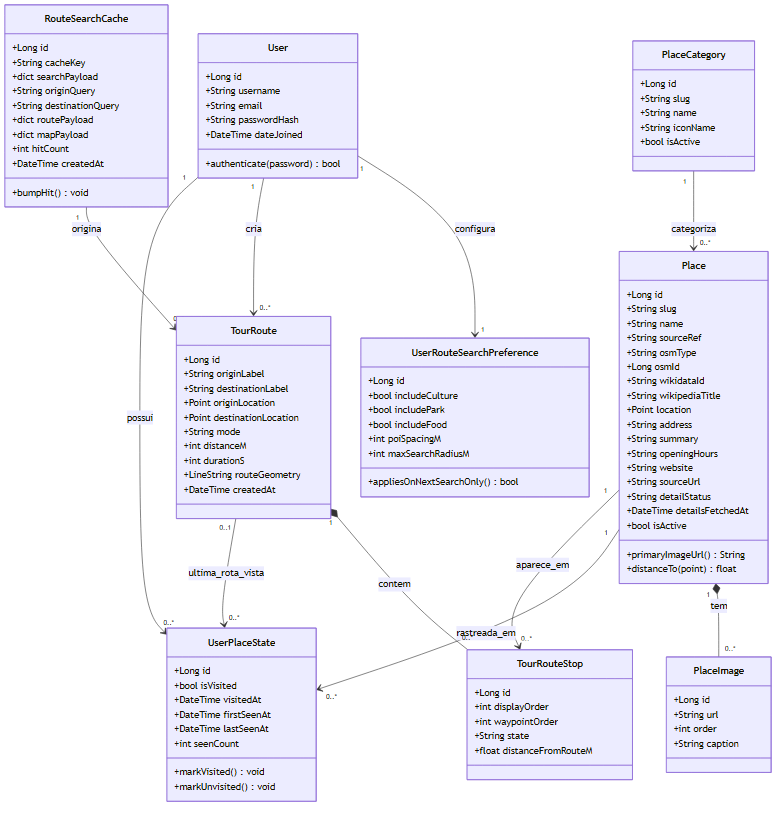
\includegraphics[width=0.95\textwidth]{figuras/classes.png}
  \caption{Diagrama de classes principal}
\end{figure}

\subsection{Casos de Uso}

\begin{figure}[H]
  \centering
  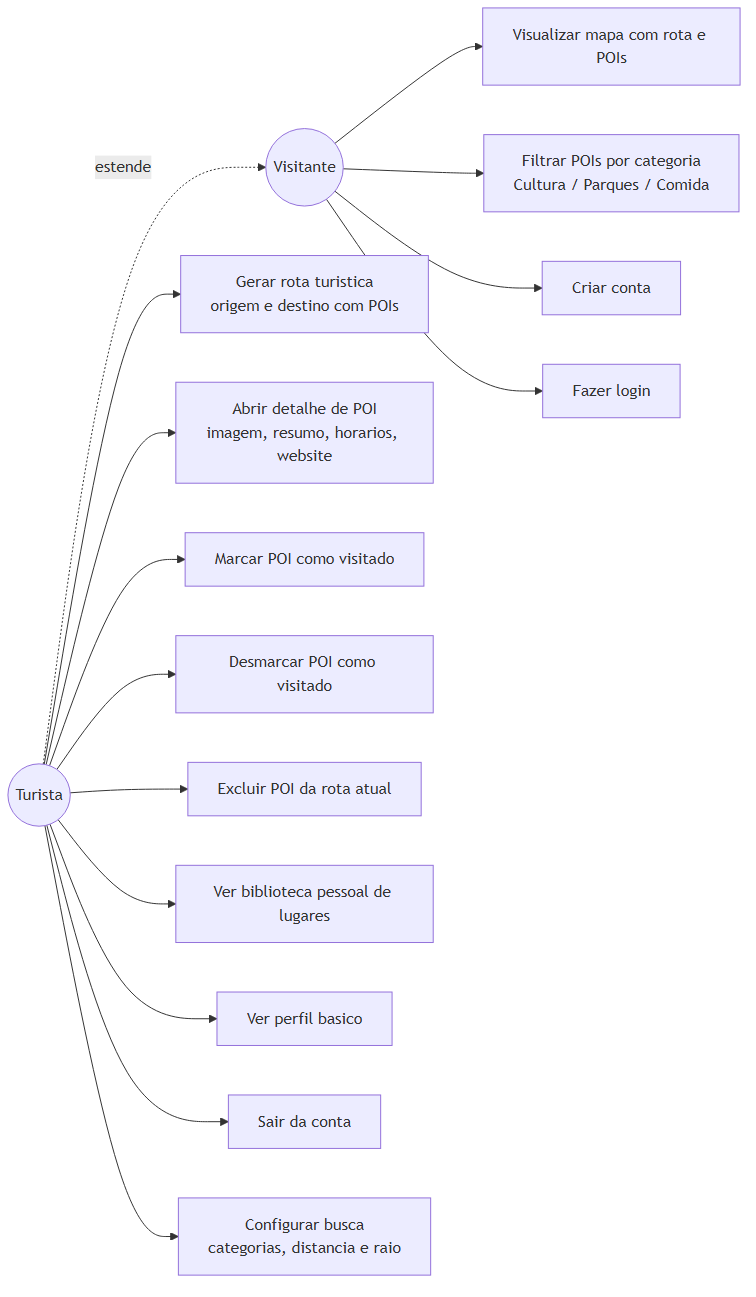
\includegraphics[height=0.72\textheight, keepaspectratio]{figuras/casos-de-uso.png}
  \caption{Diagrama de casos de uso -- MVP}
\end{figure}

O MVP define dois atores: \textbf{Visitante} (usu\'ario an\^onimo) e \textbf{Turista} (usu\'ario autenticado, que estende Visitante). O ator Administrador da proposta inicial foi removido do escopo: lugares s\~ao populados via comando \texttt{seed\_demo} e descobertos automaticamente pelo Overpass API. O ator Turista tamb\'em ganhou o caso de uso \textit{Configurar busca}, permitindo personalizar categorias, dist\^ancia entre POIs e raio m\'aximo para a pr\'oxima rota.

\subsection{Fluxos principais}

\subsubsection{Gerar Rota Tur\'istica}

\begin{figure}[H]
  \centering
  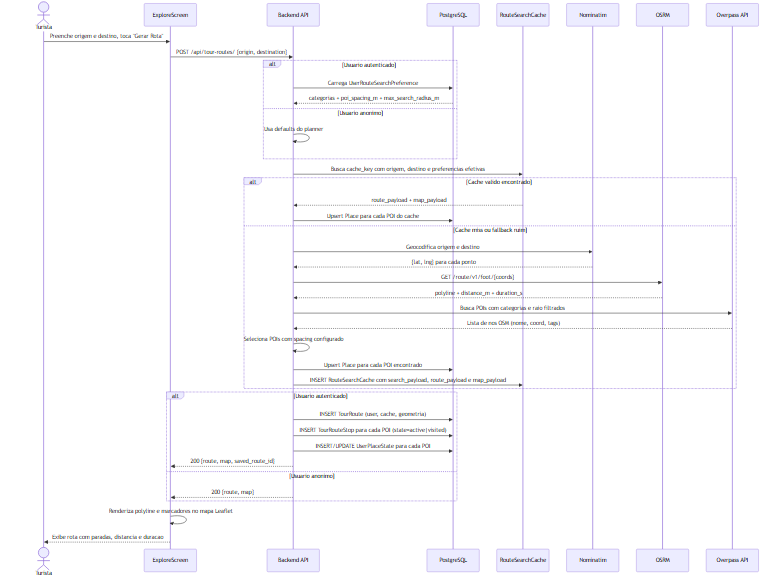
\includegraphics[width=0.95\textwidth]{figuras/sequencia-gerar-rota.png}
  \caption{Diagrama de sequ\^encia -- Gerar Rota}
\end{figure}

O fluxo de gera\c{c}\~ao de rota \'e o n\'ucleo do produto. Ao receber \texttt{POST /api/tour-routes/} com origem e destino, o backend: (1) carrega as prefer\^encias do usu\'ario autenticado ou usa os defaults do planner; (2) verifica o cache por chave can\^onica sens\'ivel a origem, destino e prefer\^encias efetivas; (3) em caso de miss, geocodifica via Nominatim, calcula rota pedestre via OSRM e busca POIs via Overpass filtrando categorias e raio; (4) aplica a heur\'istica de sele\c{c}\~ao com a dist\^ancia configurada entre paradas; (5) realiza upsert dos POIs em \texttt{Place}; (6) se o usu\'ario estiver autenticado, persiste \texttt{TourRoute}, \texttt{TourRouteStop} e \texttt{UserPlaceState} \cite{osrm2024, overpass2024}.

\subsubsection{Enriquecimento de Detalhe de POI}

\begin{figure}[H]
  \centering
  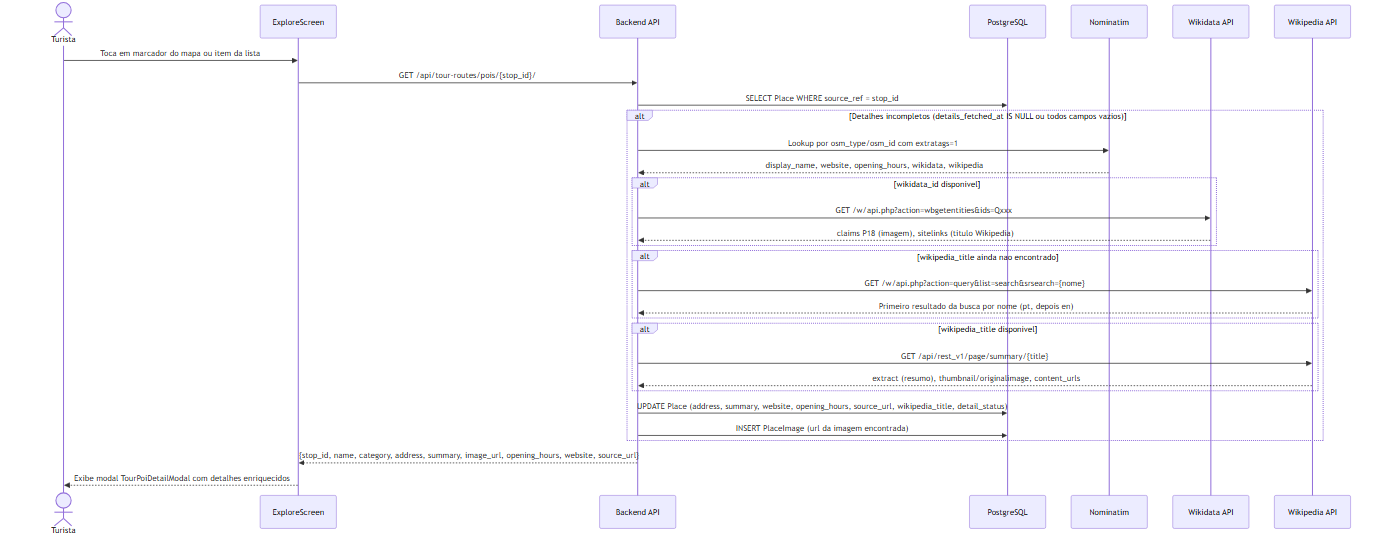
\includegraphics[width=0.95\textwidth]{figuras/sequencia-detalhe-poi.png}
  \caption{Diagrama de sequ\^encia -- Enriquecimento de detalhe de POI}
\end{figure}

Ao abrir o detalhe de um POI (\texttt{GET /api/tour-routes/pois/\{stop\_id\}/}), o backend verifica se os dados j\'a foram enriquecidos. Se n\~ao, executa a cadeia: Nominatim (extratags OSM) $\rightarrow$ Wikidata (imagem P18) $\rightarrow$ Wikipedia por nome (fallback) $\rightarrow$ Wikipedia Summary API.

\subsubsection{Marcar como Visitado}

\begin{figure}[H]
  \centering
  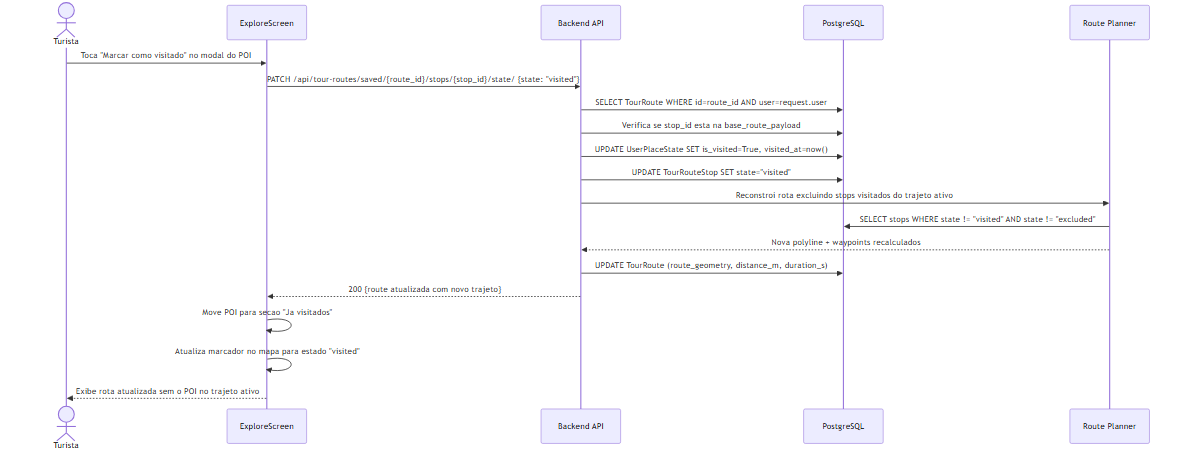
\includegraphics[width=0.85\textwidth]{figuras/sequencia-marcar-visitado.png}
  \caption{Diagrama de sequ\^encia -- Marcar como Visitado}
\end{figure}

Ao marcar um POI como visitado (\texttt{PATCH .../stops/\{stop\_id\}/state/}), o backend atualiza \texttt{UserPlaceState} e \texttt{TourRouteStop}, reconstr\'oi a rota excluindo stops visitados do trajeto ativo, e devolve a rota atualizada.

\subsubsection{Diagrama de Atividade}

\begin{figure}[H]
  \centering
  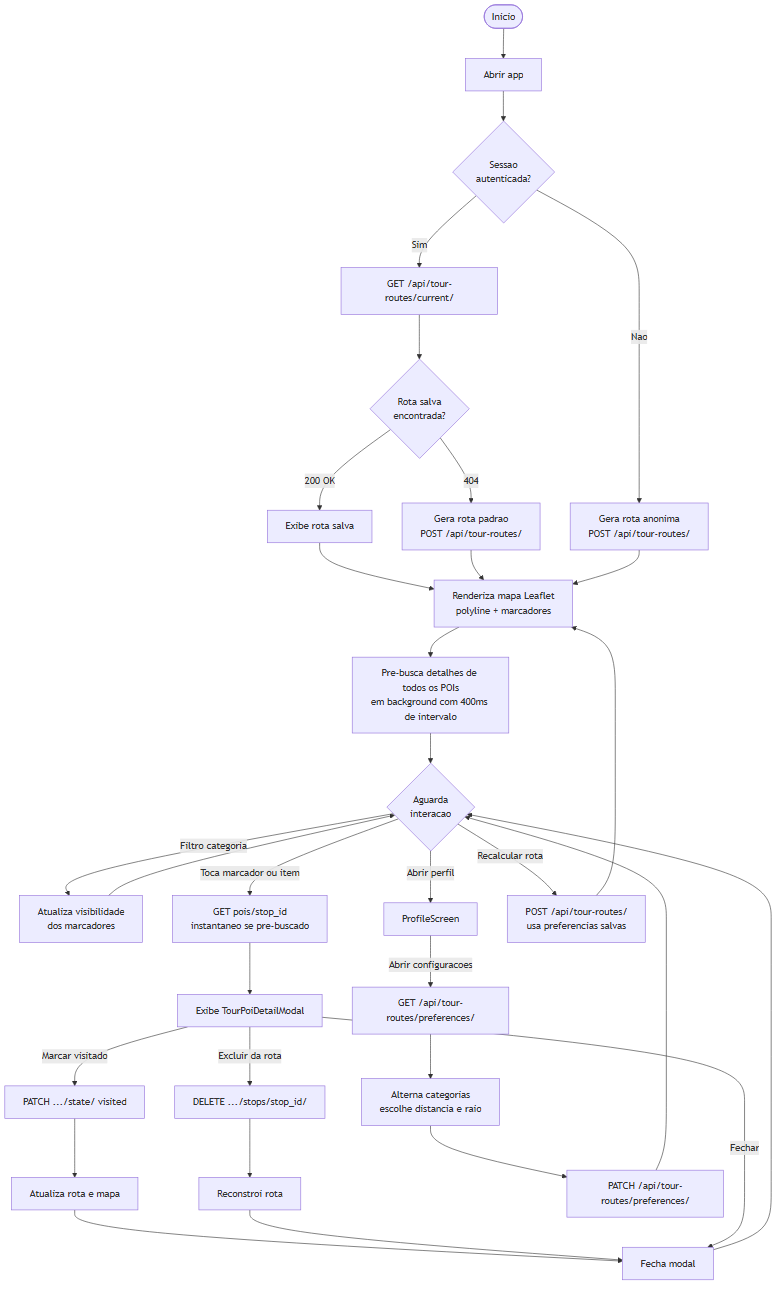
\includegraphics[height=0.82\textheight, keepaspectratio]{figuras/atividade-explorar.png}
  \caption{Diagrama de atividade -- Fluxo da ExploreScreen}
\end{figure}

\subsection{MVP Entregue}

\subsubsection{Funcionalidades implementadas}

\begin{table}[H]
\centering
\caption{Funcionalidades entregues no MVP}
\begin{tabular}{lp{9cm}}
\toprule
\textbf{Funcionalidade} & \textbf{Descri\c{c}\~ao} \\
\midrule
Autentica\c{c}\~ao JWT & Registro, login, refresh de token e logout \\
Planejamento de rota & Origem + destino com POIs selecionados ao longo do percurso \\
Mapa interativo & Leaflet via WebView/iframe com polyline, marcadores e filtros \\
Filtros de categoria & Cultura, Parques, Comida \\
Configuracoes de busca & Tela dedicada no perfil para alterar categorias, distancia entre POIs e raio maximo da proxima busca \\
Detalhe de POI & Modal com imagem, resumo, endere\c{c}o, hor\'arios, website \\
Enriquecimento autom\'atico & Imagem e resumo via Wikidata/Wikipedia \\
Marcar visitado & POI sai do trajeto ativo e vai para se\c{c}\~ao ``J\'a visitados'' \\
Excluir POI da rota & Rota recalculada sem o POI exclu\'ido \\
Biblioteca pessoal & Aba Lugares com hist\'orico de todos os POIs vistos em rotas \\
Perfil b\'asico & Dados do usu\'ario e bot\~ao de logout \\
Cache de rotas & Rota reutilizada para mesma origem/destino e mesmas prefer\^encias sem recalcular \\
\bottomrule
\end{tabular}
\end{table}

\subsubsection{Funcionalidades fora do escopo atual}

As seguintes funcionalidades identificadas na proposta inicial aguardam a defini\c{c}\~ao do modelo de monetiza\c{c}\~ao e da estrat\'egia de distribui\c{c}\~ao do produto para serem incorporadas em ciclos futuros:

\begin{itemize}
  \item Integra\c{c}\~ao com eventos culturais (Sympla, TicketMaster);
  \item Integra\c{c}\~ao com aplicativos de mobilidade (Uber, 99);
  \item Consulta de transporte p\'ublico (Quanto Tempo Falta);
  \item Sele\c{c}\~ao de modal de transporte (apenas caminhada suportada);
  \item Compra real de ingressos (endpoint mockado);
  \item Edi\c{c}\~ao de perfil de usu\'ario;
  \item Busca por voz.
\end{itemize}

\subsection{Refinamento de Escopo e Entrega do Prot\'otipo}

Ao longo do semestre, o escopo do projeto foi revisado em alinhamento com o Product Owner. A principal decis\~ao foi concentrar os esfor\c{c}os desta entrega na \textbf{valida\c{c}\~ao da arquitetura e na demonstra\c{c}\~ao de escalabilidade como MVP}, postergando para ciclos futuros as integrações com plataformas comerciais e a defini\c{c}\~ao da estrat\'egia de distribui\c{c}\~ao. Essa decis\~ao foi respaldada por tr\^es fatores:

\begin{itemize}
  \item As integrações com Sympla, TicketMaster, Uber e 99 pressup\~oem uma estrat\'egia comercial definida -- seja por comiss\~ao de transa\c{c}\~oes, parceria de visibilidade ou plano premium. Como o modelo de monetiza\c{c}\~ao do produto ainda est\'a em elabora\c{c}\~ao, incorporar essas integrações neste ciclo seria prematuro e poderia criar depend\^encias incompat\'iveis com o modelo de neg\'ocio que vier a ser adotado;
  \item A prioridade declarada pelo PO era validar a solidez da arquitetura central como funda\c{c}\~ao escal\'avel -- roteamento, enriquecimento progressivo de POIs e personaliza\c{c}\~ao de prefer\^encias -- antes de agregar camadas comerciais. Um MVP tecnicamente robusto demonstra que o produto pode suportar diferentes estrat\'egias de distribui\c{c}\~ao;
  \item Com a atua\c{c}\~ao independente do PO e a reformula\c{c}\~ao da vis\~ao do produto para uma plataforma de prop\'osito geral, o foco desta entrega se concentrou em demonstrar que a arquitetura \'e transfer\'ivel e escal\'avel al\'em de Santos, deixando a estrat\'egia de monetiza\c{c}\~ao e distribui\c{c}\~ao para a pr\'oxima fase.
\end{itemize}

Na etapa de entrega do prot\'otipo, o aplicativo foi apresentado ao PO e aos demais interessados por meio de uma reuni\~ao via Google Meet, com compartilhamento de tela e demonstra\c{c}\~ao ao vivo dos fluxos principais do aplicativo (Figura~\ref{fig:reuniao}). O feedback colhido foi positivo: o PO aprovou a arquitetura adotada, reconhecendo a robustez do sistema de roteamento com dados abertos, a coer\^encia do modelo de dados e a funcionalidade do fluxo principal de uso. Os testes realizados durante a apresenta\c{c}\~ao demonstraram comportamento satisfat\'orio nos casos de uso principais, sem inconsist\^encias cr\'iticas identificadas.

\begin{figure}[H]
  \centering
  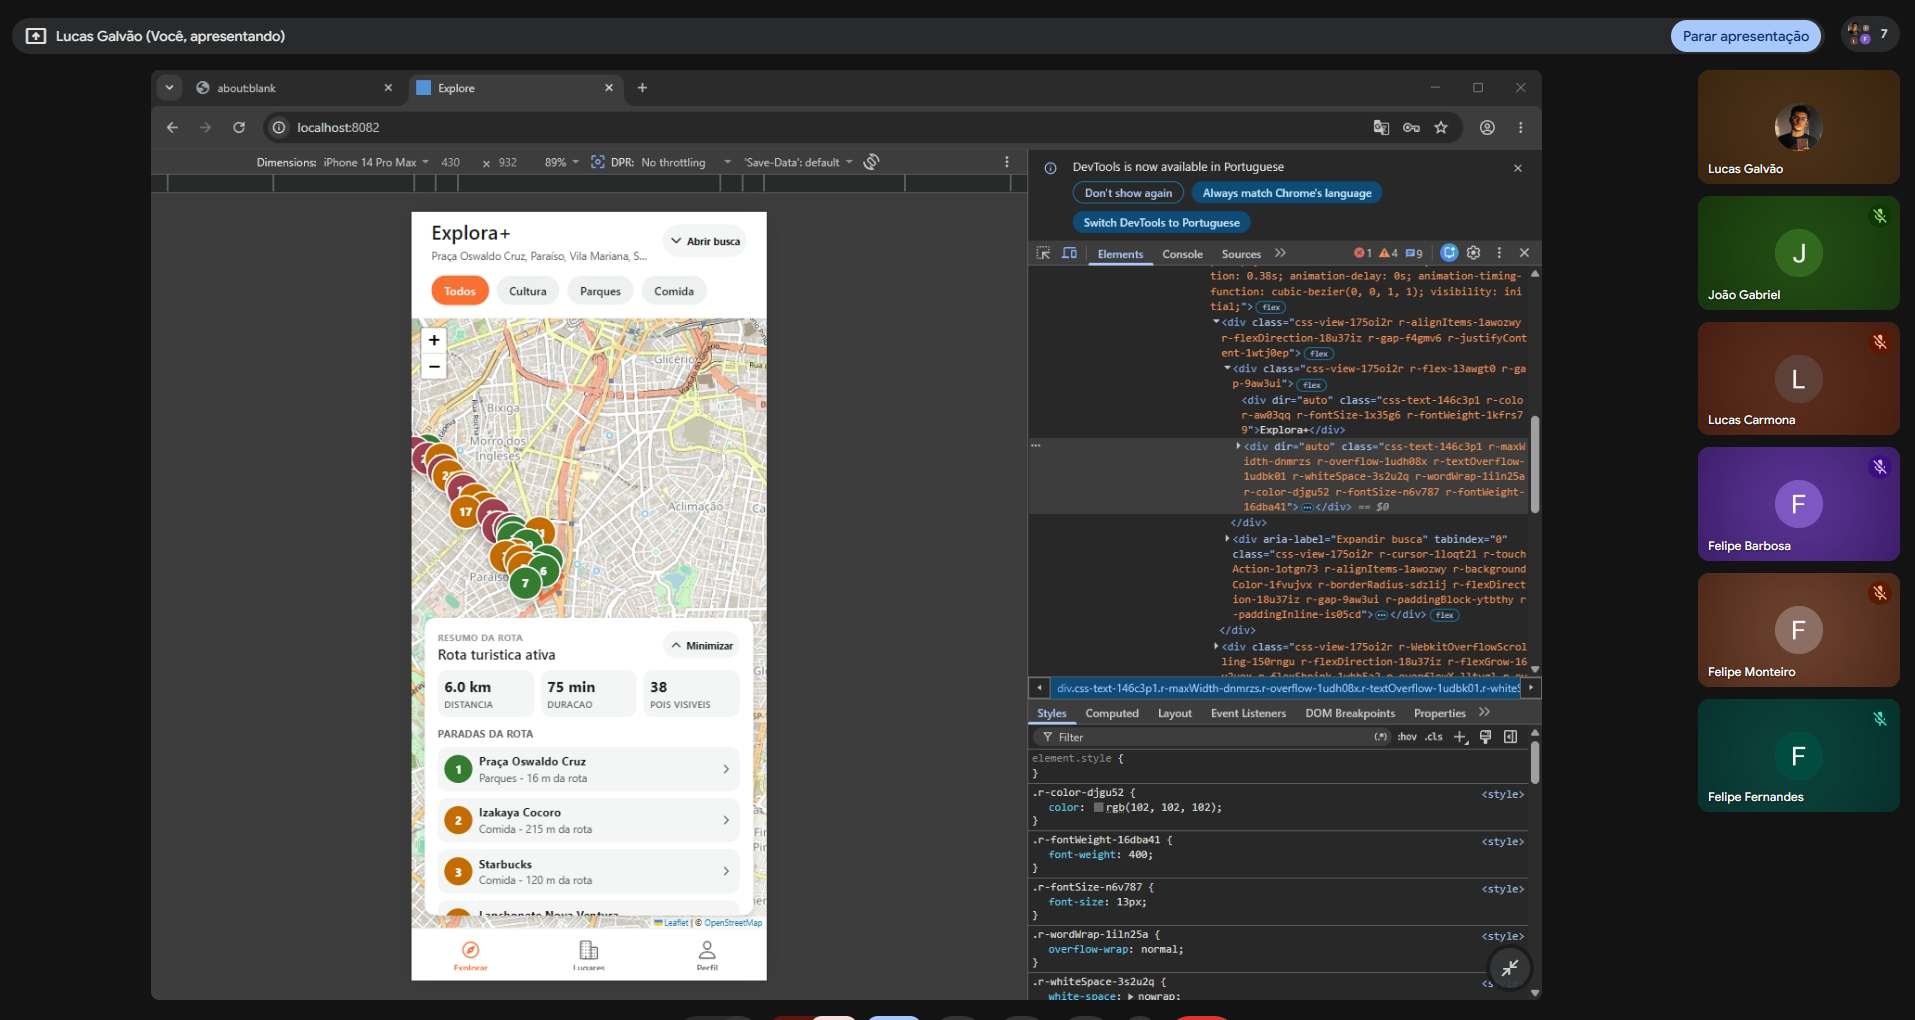
\includegraphics[width=0.95\textwidth]{figuras/reuniao.png}
  \caption{Reuni\~ao de entrega do prot\'otipo via Google Meet -- PO e equipe presentes, com demonstra\c{c}\~ao ao vivo do Explora+}
  \label{fig:reuniao}
\end{figure}

Como perspectiva de evolu\c{c}\~ao, ficou registrada a necessidade de definir um \textbf{modelo de monetiza\c{c}\~ao} para o aplicativo, etapa que viabilizar\'a as integrações com plataformas de eventos, mobilidade e transporte p\'ublico previstas na proposta original. Possibilidades levantadas incluem parcerias com estabelecimentos comerciais para destaque patrocinado de POIs em rotas, planos premium com funcionalidades avan\c{c}adas e modelos de distribui\c{c}\~ao via ag\^encias de turismo. A defini\c{c}\~ao dessa estrat\'egia \'e o pr\'oximo passo natural para levar o Explora+ de prot\'otipo validado a produto lan\c{c}ado.

% -----------------------------------------------------------
\section{Conclus\~ao}
% -----------------------------------------------------------

O Explora+ entregou uma \textbf{proposta de arquitetura validada}, demonstrando a viabilidade t\'ecnica de uma plataforma de turismo digital escal\'avel. A aprova\c{c}\~ao do PO e a demonstra\c{c}\~ao satisfat\'oria dos fluxos principais confirmam que a base est\'a pronta para suportar qualquer caminho comercial futuro, seja via parcerias, planos premium ou outros formatos a serem definidos na pr\'oxima fase.

A principal mudan\c{c}a em rela\c{c}\~ao \`a proposta inicial foi a substitui\c{c}\~ao de APIs comerciais por alternativas abertas (Nominatim, OSRM, Overpass, Wikidata, Wikipedia), tornando o sistema sustent\'avel e independente de cotas e custos. O modelo de dados evoluiu de uma rota \emph{single-destination} para um planner multi-POI com cache sens\'ivel a prefer\^encias, personaliza\c{c}\~ao por usu\'ario e enriquecimento progressivo de conte\'udo. Mais do que um prot\'otipo acad\^emico, o Explora+ demonstra que uma plataforma de descoberta tur\'istica pode ser constru\'ida sobre dados abertos globais e implantada em qualquer munic\'ipio com acervo registrado no OpenStreetMap -- o que refor\c{c}a seu car\'ater extensionista e sua transfer\'encia de impacto para al\'em de Santos.

\subsection{Justificativas t\'ecnicas das escolhas}

\begin{description}
  \item[React Native + Expo] Gera aplica\c{c}\~ao nativa para Android, iOS e Web a partir de uma \'unica base de c\'odigo, reduzindo custo de manuten\c{c}\~ao \cite{reactnative2024, expo2024}.
  \item[Django + DRF] Maturidade do framework, mapeamento ORM direto das entidades de neg\'ocio e seguran\c{c}a integrada \cite{django2024, drf2024, holovaty2009}.
  \item[PostgreSQL + PostGIS] Suporte nativo a opera\c{c}\~oes geoespaciais (dist\^ancia, proximidade, LineString) necess\'arias para roteamento e sele\c{c}\~ao de POIs \cite{postgis2024}.
  \item[OpenStreetMap + Nominatim + OSRM + Overpass] Alternativa gratuita, global e com cobertura adequada para Santos. Elimina depend\^encia de APIs pagas \cite{osm2024, nominatim2024, osrm2024, overpass2024}.
  \item[Wikidata + Wikipedia] Fonte rica de imagens e descri\c{c}\~oes culturais para pontos de interesse, sem necessidade de curadoria manual \cite{wikidata2024, wikipedia2024}.
  \item[Docker + Docker Compose] Ambiente de desenvolvimento id\^entico para todos os integrantes, com hot reload e isola\c{c}\~ao de depend\^encias \cite{docker2024, humble2010}.
\end{description}

% -----------------------------------------------------------
\printbibliography[title={Refer\^encias}]

\end{document}
